\documentclass{tufte-handout}

\title{Notizen MA3 WS 22/23}

\author[Noah Freising]{Noah Freising}

%\date{28 March 2010} % without \date command, current date is supplied

%\geometry{showframe} % display margins for debugging page layout

\usepackage{graphicx} % allow embedded images
  \setkeys{Gin}{width=\linewidth,totalheight=\textheight,keepaspectratio}
  \graphicspath{{graphics/}} % set of paths to search for images
\usepackage{amsmath}  % extended mathematics
\usepackage{booktabs} % book-quality tables
\usepackage{units}    % non-stacked fractions and better unit spacing
\usepackage{multicol} % multiple column layout facilities
\usepackage{lipsum}   % filler text
\usepackage{fancyvrb} % extended verbatim environments
\usepackage[ngerman]{babel}
  \fvset{fontsize=\normalsize}% default font size for fancy-verbatim environments

% Standardize command font styles and environments
\newcommand{\doccmd}[1]{\texttt{\textbackslash#1}}% command name -- adds backslash automatically
\newcommand{\docopt}[1]{\ensuremath{\langle}\textrm{\textit{#1}}\ensuremath{\rangle}}% optional command argument
\newcommand{\docarg}[1]{\textrm{\textit{#1}}}% (required) command argument
\newcommand{\docenv}[1]{\textsf{#1}}% environment name
\newcommand{\docpkg}[1]{\texttt{#1}}% package name
\newcommand{\doccls}[1]{\texttt{#1}}% document class name
\newcommand{\docclsopt}[1]{\texttt{#1}}% document class option name
\newenvironment{docspec}{\begin{quote}\noindent}{\end{quote}}% command specification environment

% ================ BEISPIELE ===================

\usepackage{amsthm}
\usepackage{xcolor}

\newtheoremstyle{own}%
    {3pt}% Space above
    {3pt}% Space below
    {}% Body font
    {}% Indent amount
    {\textbf}% Theorem head font
    {:}% Punctuation after theorem head
    {\newline}% Space after theorem head
    {}% Theorem head spec

\theoremstyle{own}
\newtheorem{example}{Beispiel}[]

\begin{document}

\maketitle% this prints the handout title, author, and date

\begin{abstract}
\noindent
Notizen zur Vorlesung MA3 im Studiengang IB an der Hochschule Mannheim. Gehalten im Wintersemester 2022/23.
\end{abstract}

{\small\tableofcontents}

%\printclassoptions

\section{Kombinatorik}

\section{Verteilungen}

Eine Verteilungsfunktion hat den Aufbau:

\begin{align}
F = & P(X \leq x) \label{defver:1} \\ 
F  :&  \mathbb{R} \mapsto [0;1] \label{defver:2}
\end{align}

$F$ bildet also die Wahrscheinlichkeit für alle Werte der Zufallsvariablen $X$ für $X \leq x$ ab \eqref{defver:1}. Dabei wird für jedes $x$ eine Wahrscheinlichkeit abgebildet.

\section{Diskrete Verteilungen}

\subsection{Binomialverteilung}

\section{Stetige Verteilungen}

Die Dichtefunktion\footnote{Die Dichtefunktion ist das \textit{stetige} Gegenstück zur \textit{diskreten} Verteilungsfunktion}
einer stetigen Verteilung zeichnet sich, wie der Name impliziert durch das Vorhandensein eines Wert an allen Stellen aus
\footnote{Der Definitionsbereich ist $\mathbb{R}$.}. 
Wir nutzen hier anstelle einer Verteilungsfunktion eine Dichtefunktion
\footnote{Das Integral bis $x$ stellt die Wahrscheinlichkeit $P(X \leq x)$ dar.}:

\begin{equation}
	\int_{-\infty}^x f(t) dt 
\end{equation}

Damit es sich um eine Dichtefunktion einer Verteilung handelt, müssen zwei Eigenschaften erfüllt sein:
\marginnote{

\eqref{dichteeig:1}: Wahrscheinlichkeiten können nicht negativ sein

\eqref{dichteeig:2}: Insgesamt beträgt die kumulierte Wahrscheinlichkeit 1
}
\begin{align}
&f(t) \geq 0 \hspace{1em} \forall t \in \mathbb{R} \label{dichteeig:1}\\
&\int_{-\infty}^{\infty} f(t) dt =1 \label{dichteeig:2}
\end{align}

\subsection{Gleichverteilung}

Bei einer Gleichverteilung definieren wir die Dichtefunktion:

\begin{equation}
f(x) = \begin{cases}
\frac{1}{b-a} \hspace{1em} &\text{für} \hspace{1em} x \in [a,b] \\
0 \hspace{1em} &\text{sonst}
\end{cases}
\end{equation}

\begin{marginfigure}
	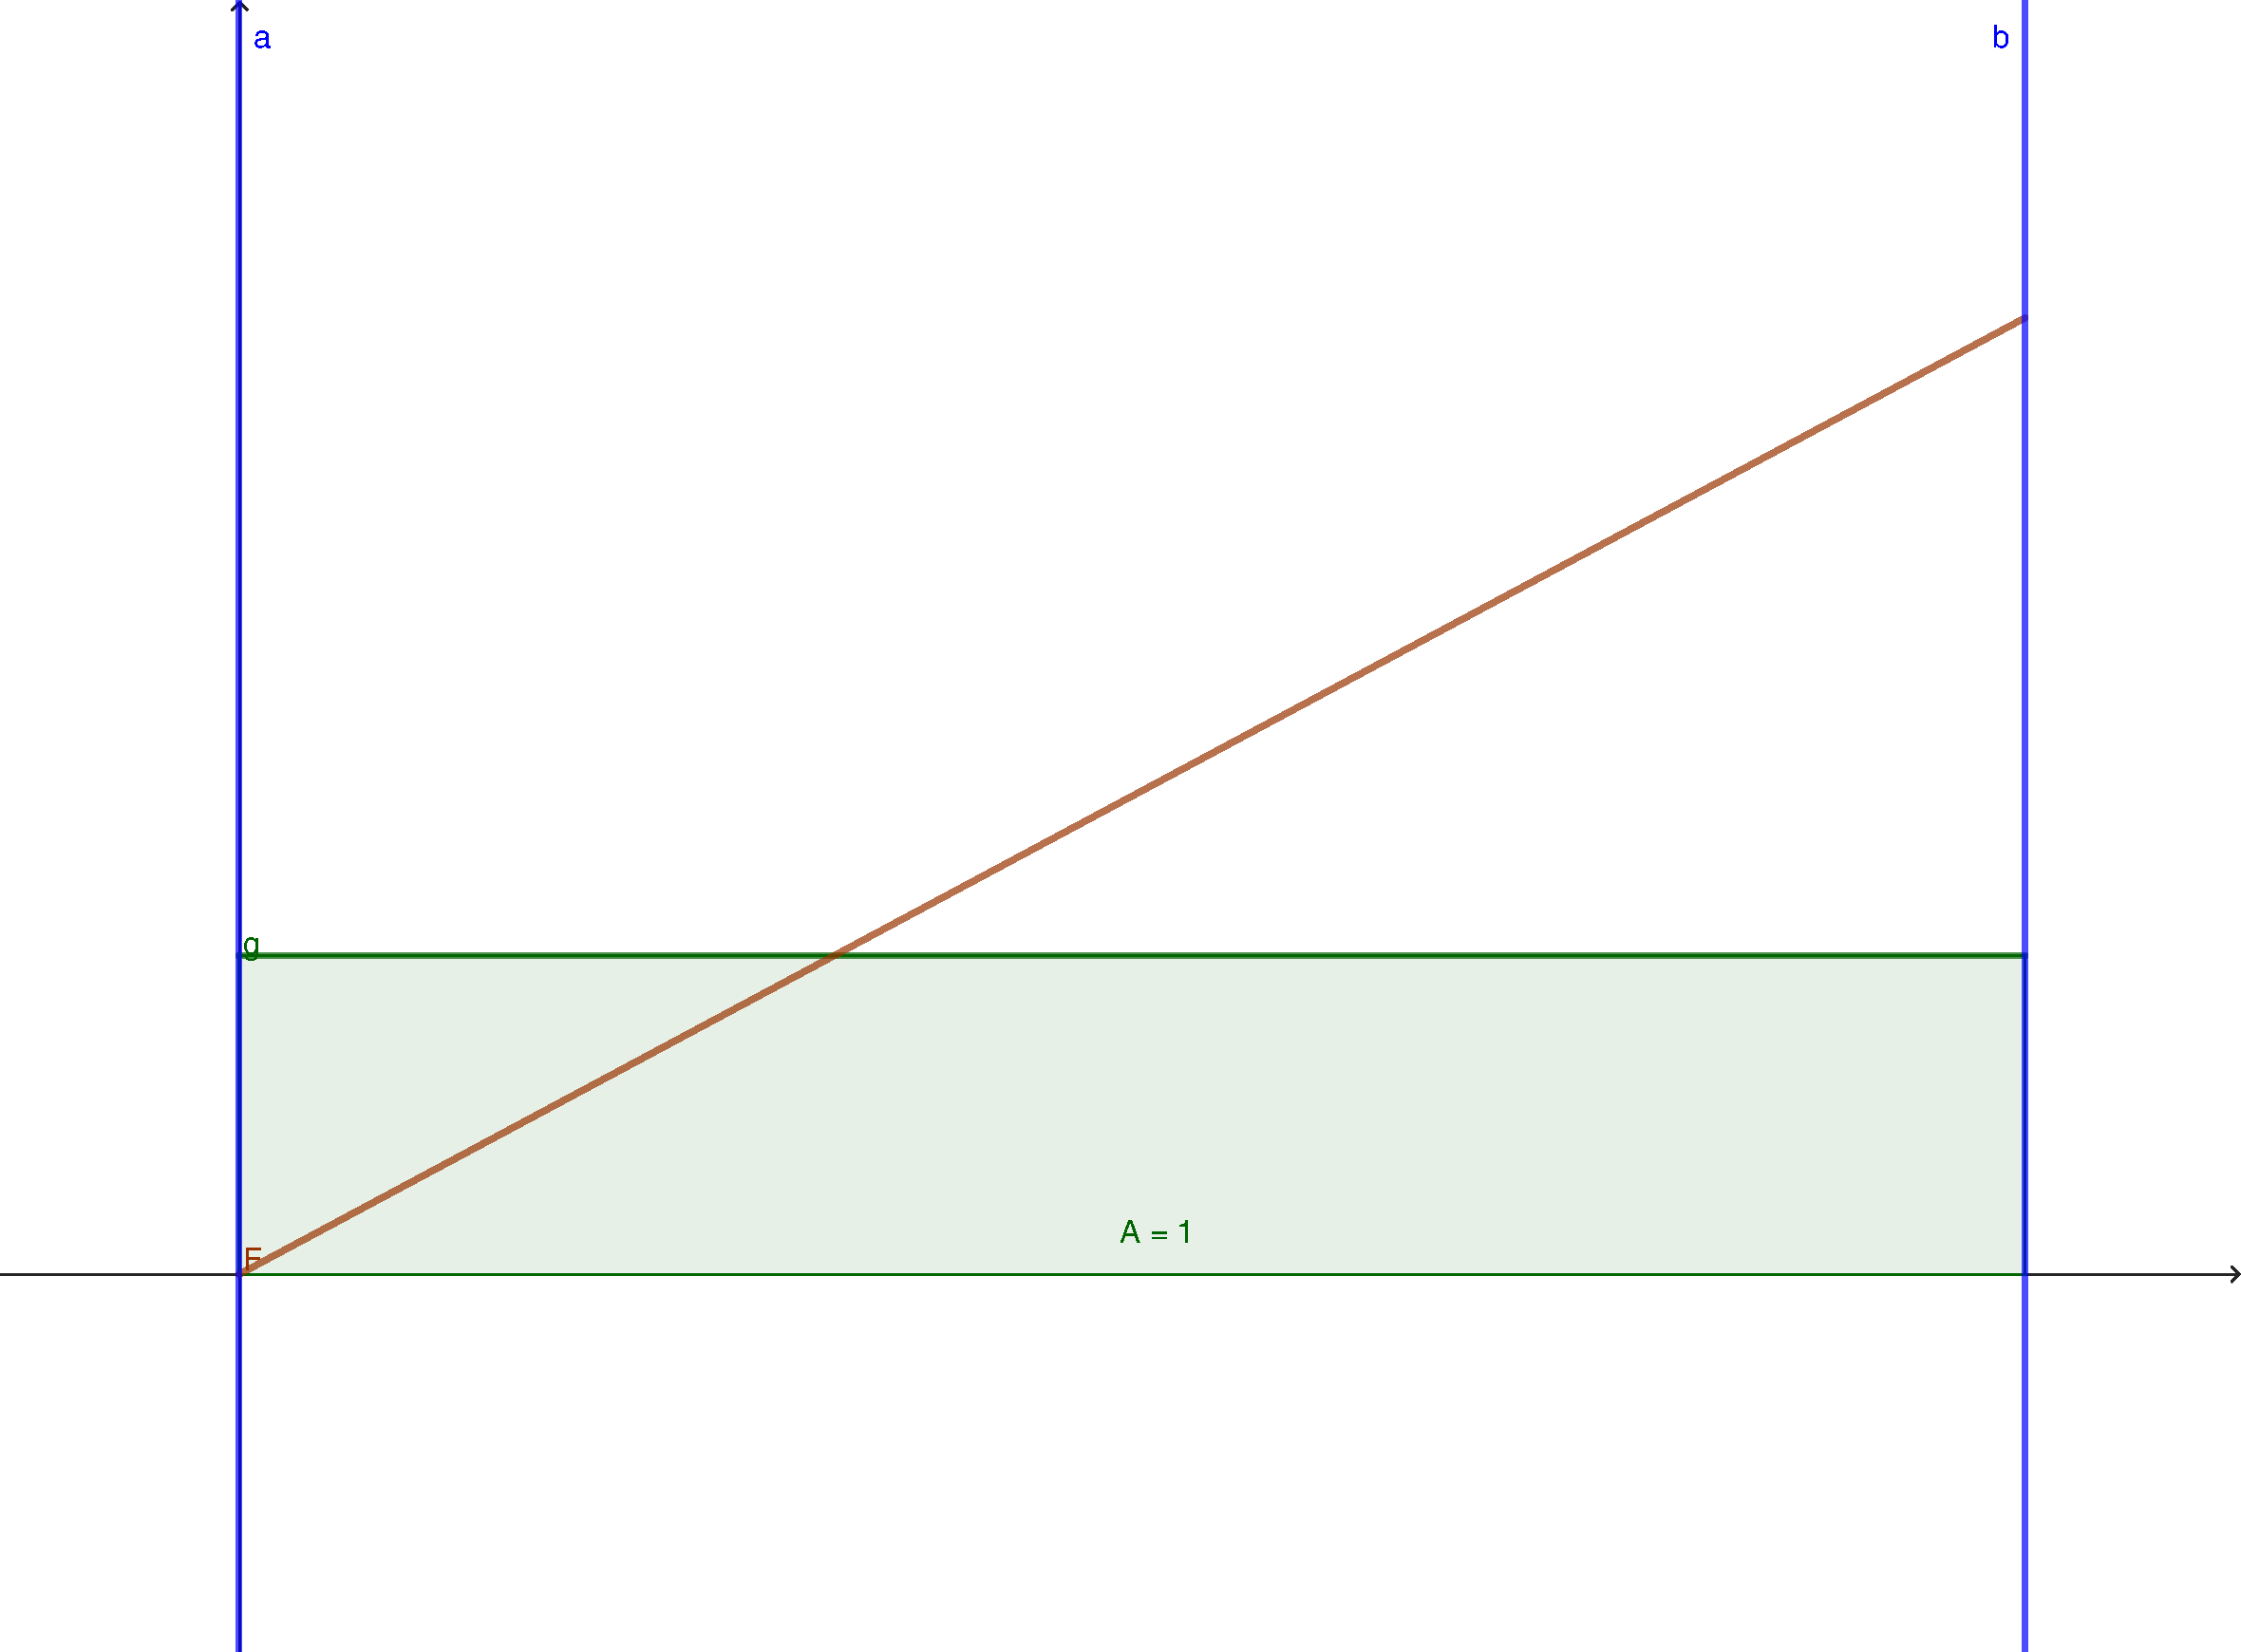
\includegraphics{gleichverteilung}
	\caption{Beispiel einer Gleichverteilung}
\end{marginfigure}

Die Wahrscheinlichkeiten berechnen sich:

\begin{equation}
P(X\leq x) = F(X) = \begin{cases}
0 \hspace{1em} & \text{für}  \hspace{1em} x < a \\
\frac{x-a}{b-a} \hspace{1em} & \text{für}  \hspace{1em} a \leq x \leq b \\
1 \hspace{1em} & \text{für}  \hspace{1em} x > b
\end{cases}
\end{equation}

\subsection{Exponentielle Verteilung}

Die Dichtefunktion einer exponentiellen Verteilung hat die Form:

\begin{equation}
	f(x) = \lambda \cdot e^{-\lambda x}
\end{equation}

Nach Bedingung \eqref{dichteeig:2} müssen wir zeigen, dass
$\int_{-\infty}^\infty = 1$.\footnote{Da wir mit einer Exponentialfunktion arbeiten, die wir für $x\geq0$ definieren, beweisen wir analog $\int_0^\infty = 1$.}

\begin{proof}
\begin{align*}
\int_0^\infty f(t) dt &= \lambda \int_0^\infty e^{-\lambda t} dt = \lambda \cdot [\frac{e^{-\lambda t}}{- \lambda}]_0^\infty \\
	&= [-e^{-\lambda t}]_0^\infty = -0 - (-1) = 1
\end{align*}
\end{proof}

\begin{marginfigure}
	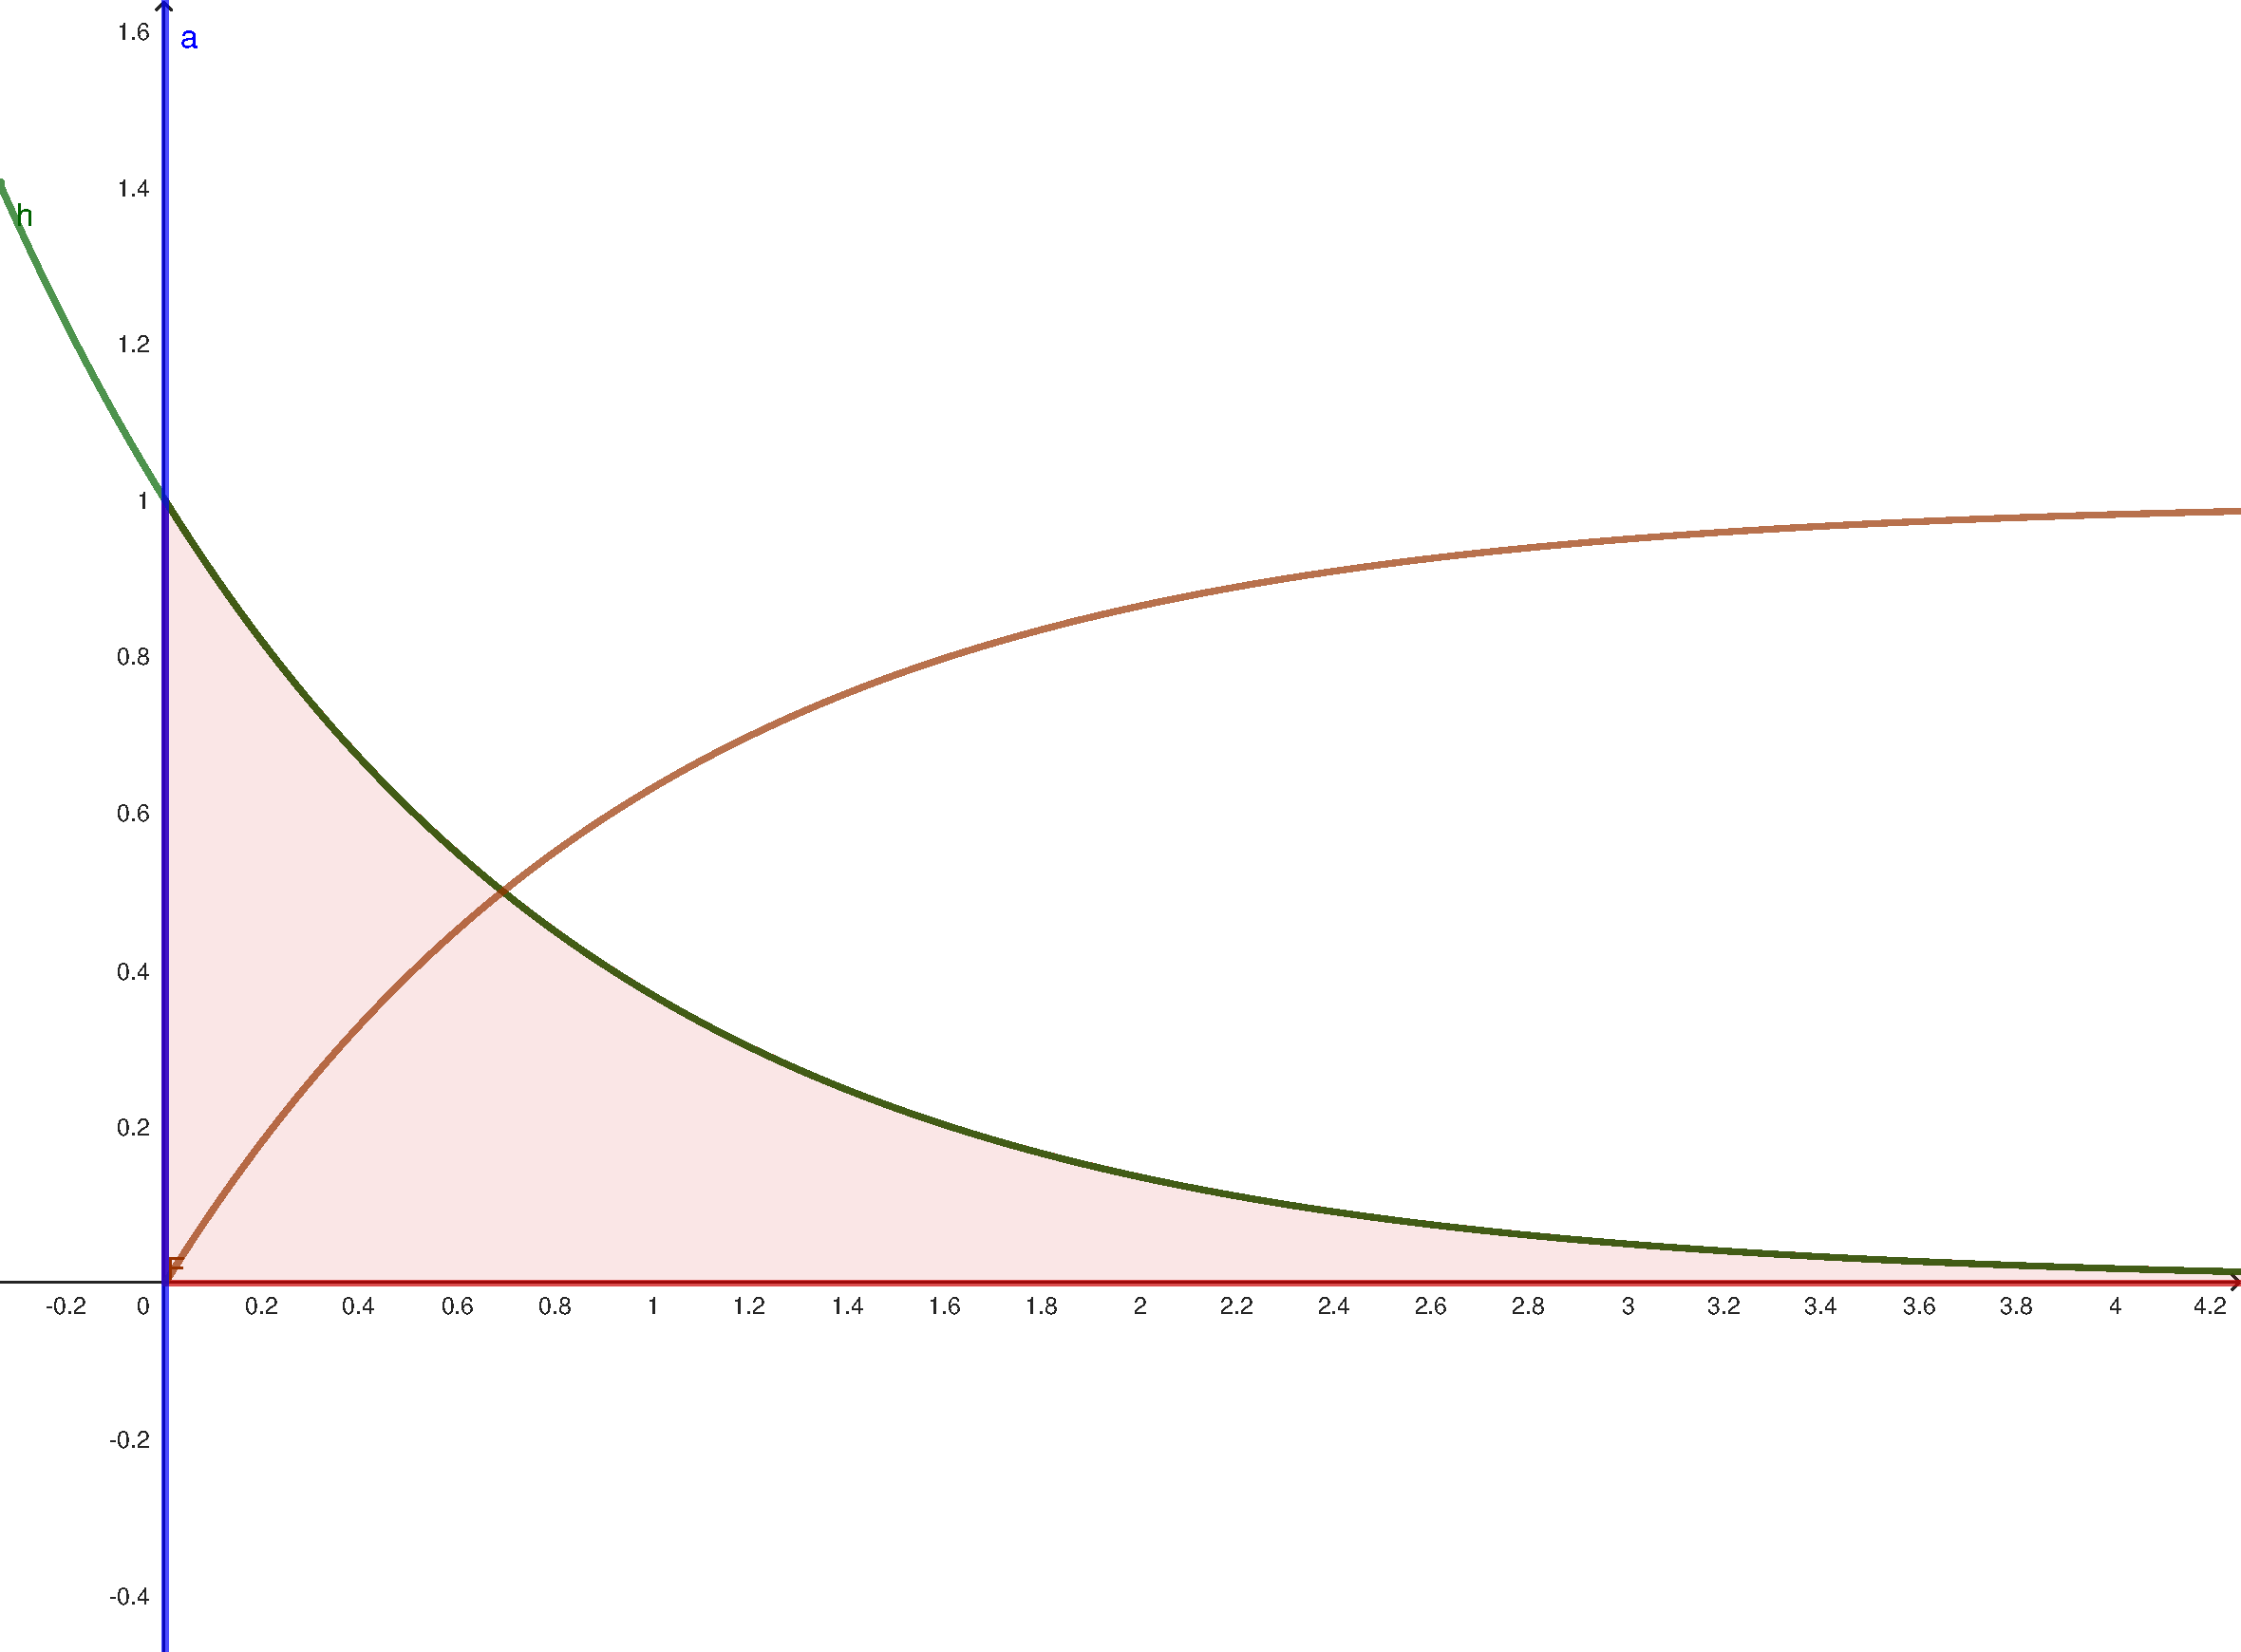
\includegraphics{exponentialverteilung}
	\caption{Beispiel einer Exponentialverteilung}
\end{marginfigure}

Die entsprechende Wahrscheinlichkeitsfunktion:

\begin{equation}
F(x) = \begin{cases}
1 - e^{- \lambda x} \hspace{1em} & \text{für} \hspace{1em} x >0 \\
0 \hspace{1em} & \text{für} \hspace{1em} x \leq 0
\end{cases}
\end{equation}

\subsection{Normalverteilung}

Die Normalverteilung folgt der grundlegenden Form $f(t) = e^{- t^2}$. Überprüfen wir zunächst
die Eigenschaften \eqref{dichteeig:1}\footnote{trivial, $e^0 = 1$} und \eqref{dichteeig:2}.

\begin{marginfigure}
	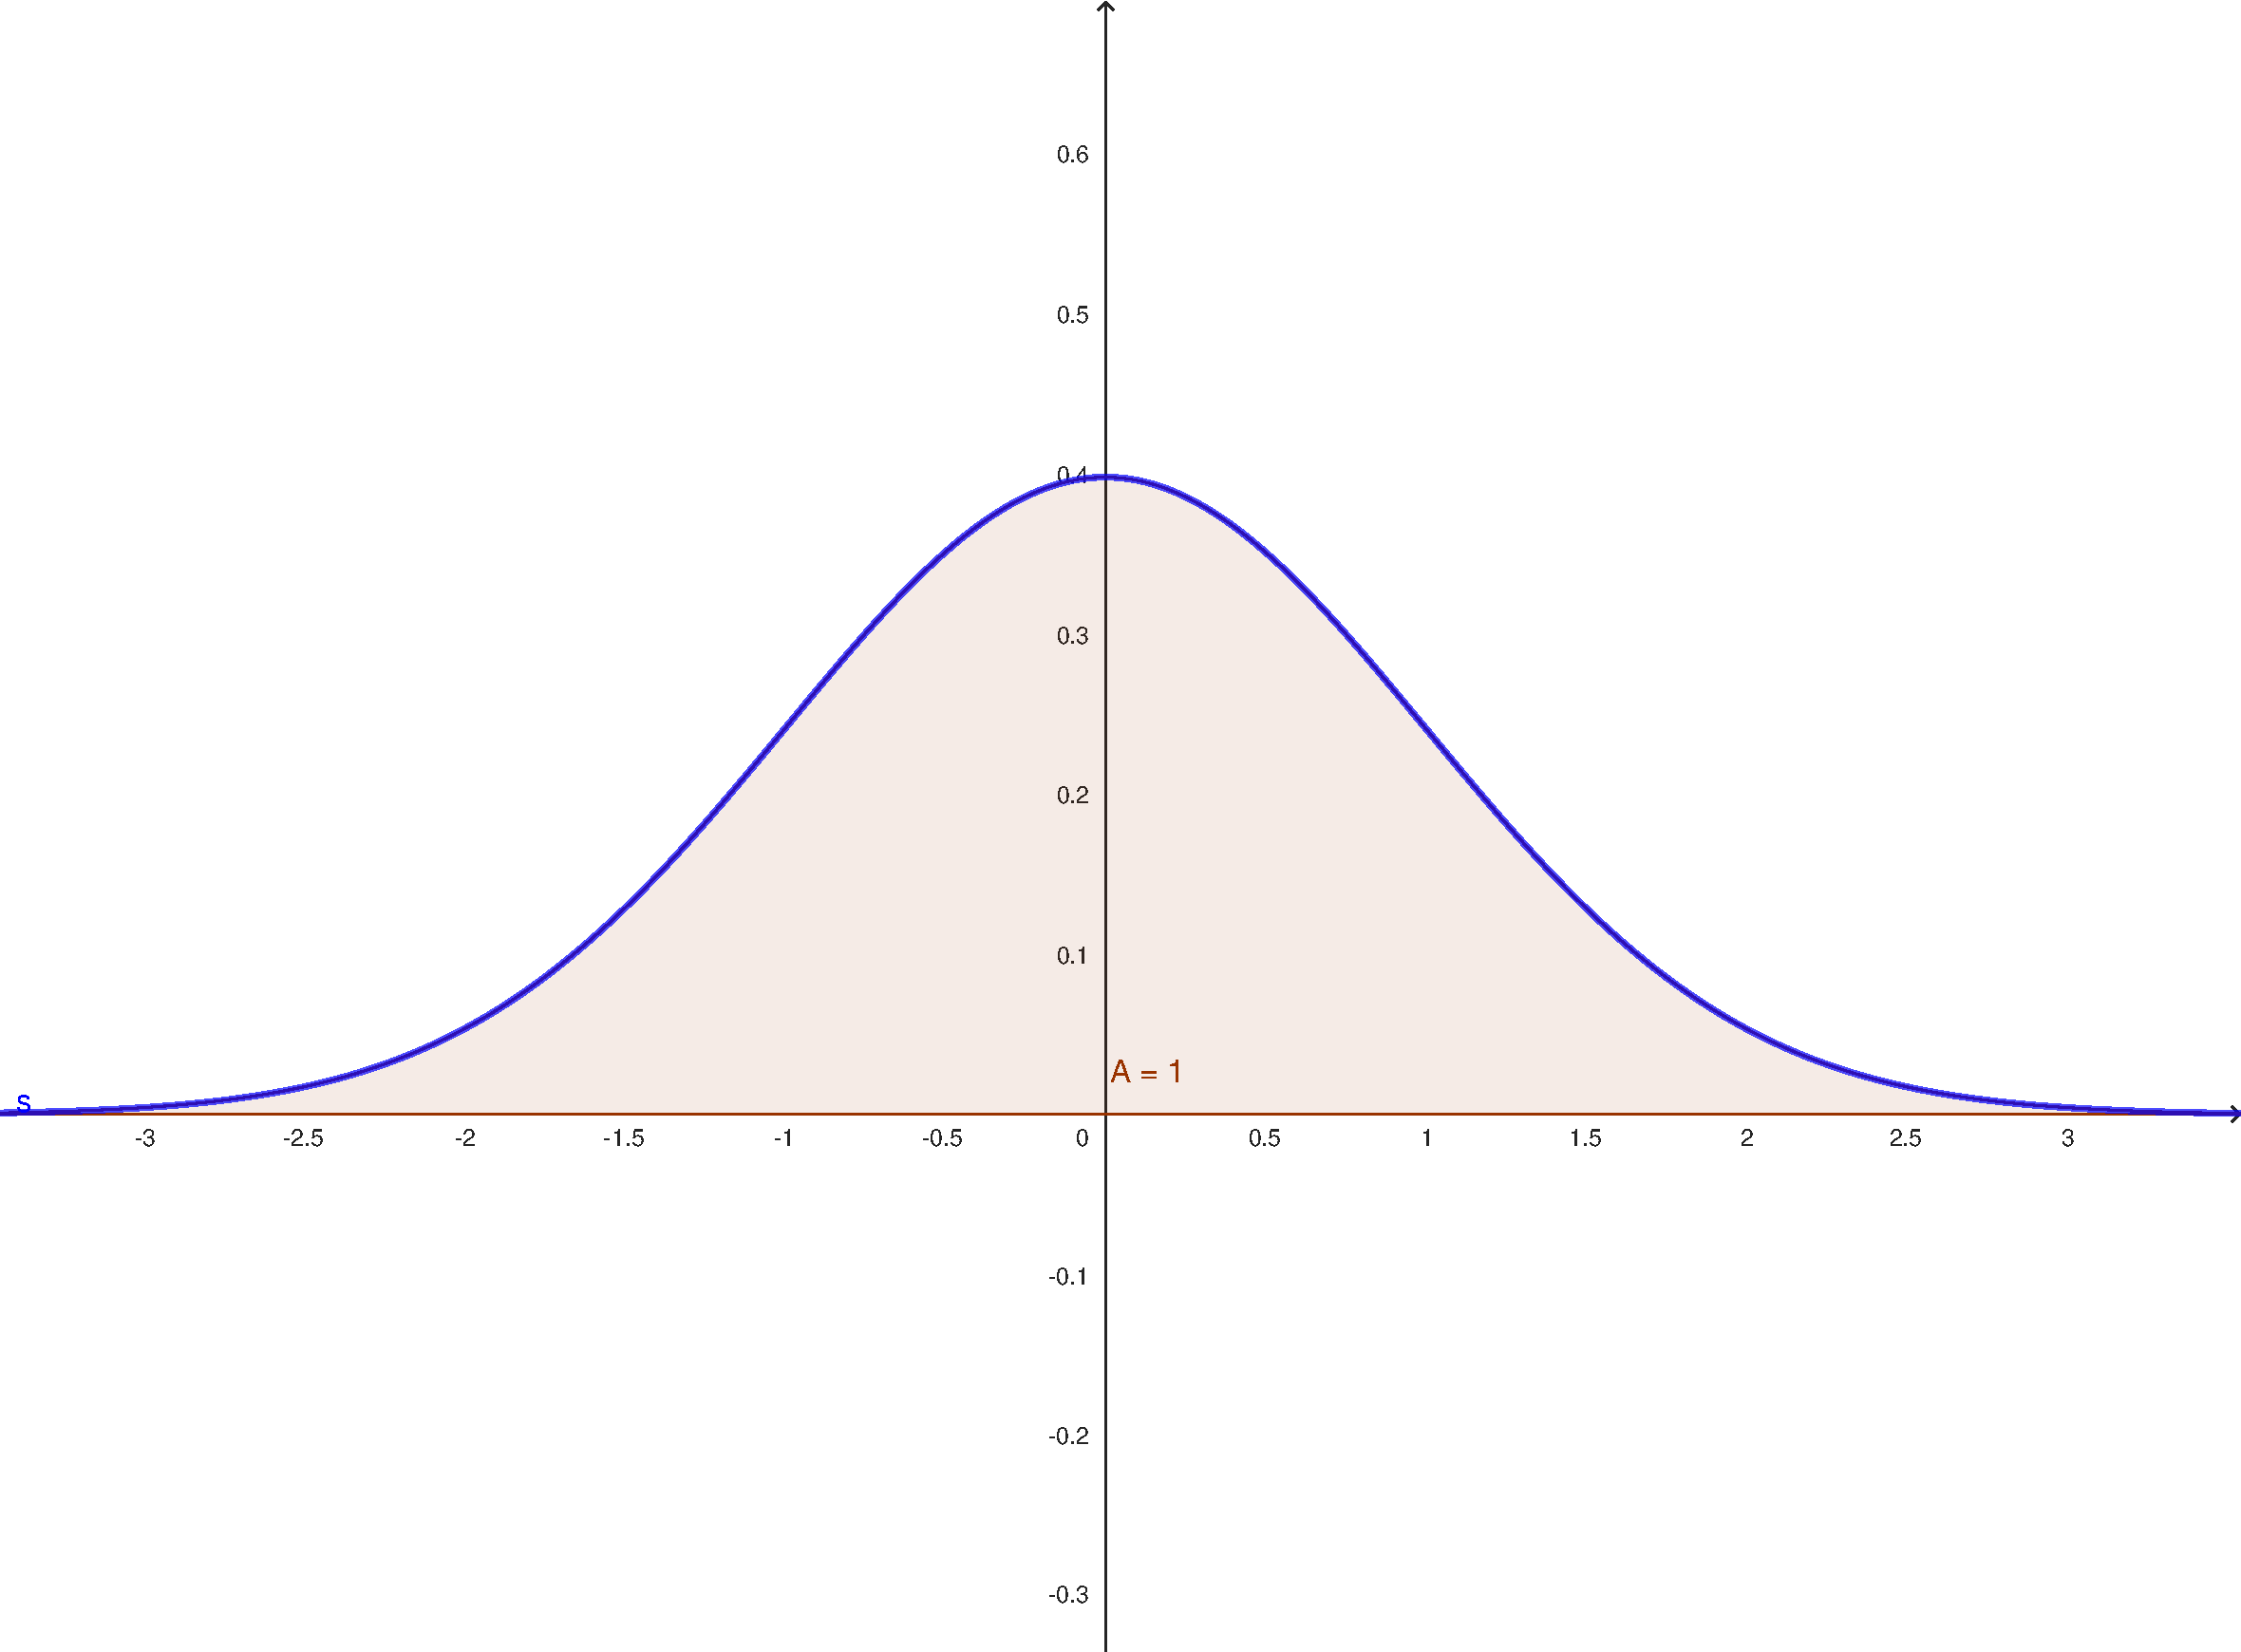
\includegraphics{normalverteilung}
	\caption{Beispiel einer Normalverteilung}
\end{marginfigure}

Zu \eqref{dichteeig:2}:

\begin{gather*}
	\int_{-\infty}^\infty e^{\frac{- t^2}{2}} dt = \sqrt{2 \Pi}
\end{gather*}

Da $\sqrt{2\Pi} > 1$, ist Bedingung \eqref{dichteeig:2} nicht erfüllt. Wir definieren daher die \textit{Standard-Normalverteilung} $\phi$ wie folgt
\footnote{Wir normieren die Funktion auf das berechnete Integral, damit $\int_{-\infty}^\infty = 1$}:

\begin{equation}
\phi(t) = \frac{e^{\frac{-t^2}{2}}}{\sqrt{2 \Pi}}
\end{equation}

Zusätzlich definieren wir die \textit{allgemeine Normalverteilung}
\footnote{
$\mu$: Verschiebung entlang der x-Achse \\
$\sigma$: Stauchung/Streckung}:

\begin{equation}
\phi(t) = \frac{1}{\sqrt{2 \Pi} \sigma} \cdot e^{- \frac{1}{2} (\frac{x - \mu}{\sigma})^2}
\end{equation}

\subsection{Unabhängigkeit zweier Zufallsvariablen}

Sei $(\Omega, P)$ ein Wahrscheinlichkeitsraum und $X,Y : \Omega \mapsto \mathbb{R}$ zwei Zufallsgrößen.
$X$ und $Y$ heißen \textit{unabhängig}, wenn $\forall x \in W(X), y \in W(Y)$:

\begin{equation}
	P(X=x, Y=y) = P(X=x) \cdot P(Y=y)
\end{equation}

gilt. Bei gemeinsamen Verteilungen sprechen wir von \textit{diskreten} Zufallsvariablen.

\begin{marginfigure}
  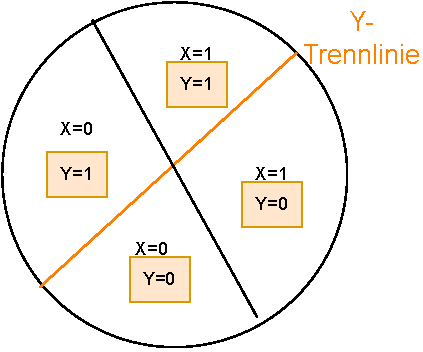
\includegraphics{zweizufallsvariablen}
  \caption{Mögliche Kombinationen zweier Zufallsvariablen in $\Omega$.}
\end{marginfigure}

\begin{example}
Beispiel einer unabhängigen, gemeinsamen Verteilung.
Hier sehen wir das
an der Vierfeldertafel\footnote{Siehe Beispielsweise: $P(X=0,Y=0) = P(X) \cdot P(Y) = \frac{1}{4} \cdot \frac{1}{4} = \frac{1}{16}$}:

\begin{center}
\begin{tabular}{l|lll}
 X/Y&  Y=0 &  Y=1  &   \\
\hline
 X=0& $\frac{1}{16}$ & $\frac{3}{16}$ & 0.25  \\
X=1 & $\frac{3}{16}$  &  $\frac{9}{16}$ &  0.75  \\
 &  0.25 & 0.75  & 1 
\end{tabular}
\end{center}
\end{example}

Die Wahrscheinlichkeitsverteilung einer diskreten 2-dimensionalen
Zufallsgröße lässt sich durch die Wahrscheinlichkeitsfunktion

\begin{equation}
f(x) = \begin{cases}
P_{ik} \hspace{1em} \text{falls}  \hspace{1em} x=x_i, y =y_k \\
0 \hspace{1em} \text{sonst}
\end{cases}
\end{equation}

darstellen.

\section{Erwartungswert}

Für eine \textit{diskrete} Zufallsgröße ist der Erwartungswert

\begin{equation}
E(X) = \sum_i x_i P(X=x_i).
\end{equation}

\begin{example}\label{bsp:erwartungswertdiskret}
 Erwartungswert einer gegebenen Wahrscheinlichkeitsverteilung


\begin{center}
\begin{tabular}{l|llllll}
 $x_i$&  0 & 2 & 3 & 4 & 10 & 11  \\ \hline
 $p_i$&  $\frac{3}{8}$ & $\frac{1}{8}$ & $\frac{1}{8}$ & $\frac{1}{8}$ & $\frac{1}{8}$ & $\frac{1}{8}$
\end{tabular}
\end{center}

\begin{gather*}
E(X) = 0 \cdot \frac{3}{8} + 2 \cdot \frac{1}{8} + 3 \cdot \frac{1}{8} + 4 \cdot \frac{1}{8} + 10 \cdot \frac{1}{8} + 11 \cdot \frac{1}{8}
\end{gather*}

\end{example}

Für eine \textit{stetige} Zufallsgröße ist der Erwartungswert
\footnote{Funktioniert prinzipiell genau wie im \textit{diskreten}, aber mit Integral statt Summe}:

\begin{equation}
E(X) = \int_{-\infty}^{\infty} y \cdot f(y) dy
\end{equation}

\begin{example}\label{bsp:erwartungswertstetig}
Erwartungswert einer stetigen Verteilung\footnote{gerne in Klausuren gefragt}

\begin{equation*}
	f(x) = \begin{cases} 
	ax^2, 0 \leq x \leq 5 \\
	0, \text{sonst}
	\end{cases}
\end{equation*}

\begin{gather*}
\int_{-\infty}^{\infty} f(x)dx = \int_0^5 ax^2 dx = 1 \\
[\frac{a x^3}{3}]_0^5 = \frac{125a}{3} - \frac{0a}{3} =  \frac{125a}{3} = 1 \\
a = \frac{3}{125}
\end{gather*}

Der Erwartungswert ist dann:

\begin{gather*}
E(X) = \int_0^5 x \frac{3}{125} x^2 dx \\
= [\frac{3}{125} \cdot \frac{x^4}{4}]_0^5 = \frac{3}{125} \cdot {625}{4} = \frac{15}{4}
\end{gather*}

\end{example}

\subsection{Rechenregeln für den Erwartungswert}

Sei $(\Omega, P)$ ein Wahrscheinlichkeitsraum und $X,Y : \Omega \mapsto \mathbb{R}$ zwei Zufallsgrößen. Es gilt:

\begin{gather}
E(X + Y) = E(X) + E(Y) \\
E( a \cdot X + b \cdot Y) = a \cdot E(X) + b \cdot E(Y)  \\
\text{Sind X , Y unabhängig dann gilt} \hspace{1em} E (X \cdot Y ) = E ( X )\cdot E ( Y )
\end{gather}

\section{Varianz}

Der mittlere Abstand der Werte vom Erwartungswert. Die quadratische Funktion ist besser als der Betrag analytisch.

Die Varianz zum Beispiel \autoref{bsp:erwartungswertdiskret}:

\begin{gather*}
Var(X) = - \frac{15}{4} ^2 \frac{3}{8} + \frac{-7}{4}^2 \frac{1}{8} + \frac{-3}{4}^2 \frac{1}{8} + \frac{1}{4}^2 \frac{1}{8} + \frac{25}{4}^2 \frac{1}{8} + \frac{28}{4}^2 \frac{1}{8}
\end{gather*}

Die Varianz zum Beispiel \ref{bsp:erwartungswertstetig}:

\begin{gather*}
	f(x) = \begin{cases} 
	\frac{3}{125}x^2, 0 \leq x \leq 5 \\
	0, \text{sonst}
	\end{cases} \\
	E(X) = \frac{15}{4} \\
	Var(X) = \int_{-\infty}^\infty (x - \frac{15}{4})^2 f(x) dx \\
	= \int_0^5 (x - \frac{15}{4})^2 \frac{3}{125} x^2 dx
\end{gather*}

Die Varianz lässt sich so (einfacher) auch so berechnen:\footnote{Das ist nicht besser, aber einfacher. Nicht die schöne Definition, sondern den schnellen Weg wählen.}

\begin{equation}
\label{var:einfach}
Var(X) = E(X^2) - (E(X))^2 
\end{equation}

\begin{proof}
\begin{align*}
Var(X) :&= E((X - E(X))^2) \\
&= E(X^2 - 2E(X) \cdot X  + (E(X))^2) \\
&= E(X^2) - E(2E(X)\cdot X) + E((E(X))^2) \\
&= E(X^2) - E(X)E(X) + (E(X))^2 \\
&= E(X^2) - (E(X))^2
\end{align*}
\end{proof}




\marginnote{
\begin{tabular}{l|llllll}
 $x_i$&  0 & 2 & 3 & 4 & 10 & 11  \\ \hline
 $p_i$&  $\frac{3}{8}$ & $\frac{1}{8}$ & $\frac{1}{8}$ & $\frac{1}{8}$ & $\frac{1}{8}$ & $\frac{1}{8}$ \\ \hline
 $x_i^2$& 0 & 4 & 9 & 16 & 100 & 121
\end{tabular}

aktualisierte Tabelle zu Beispiel \ref{bsp:erwartungswertdiskret}
}


Die Varianz zum Beispiel \autoref{bsp:erwartungswertdiskret}:

\begin{gather*}
Var(X) = \frac{250}{8} - \frac{15^2}{4^2} = \frac{500-225}{16} = \frac{225}{16}
\end{gather*}

Die Varianz zum Beispiel \autoref{bsp:erwartungswertstetig}:

\begin{gather*}
E(X^2) = \int_{-\infty}^\infty x^2 f(x) dx = \frac{3}{125} \int_0^5 x^2 x^2 dx \\
= \frac{3}{125} [\frac{x^5}{5}]_0^5 = 15.
\end{gather*}

\begin{gather*}
Var(X) = 15 - (\frac{15}{4})^2 = \frac{15 \cdot 16 - 15^2}{16} = \frac{15}{16}.
\end{gather*}


\bibliography{sample-handout}
\bibliographystyle{plainnat}



\end{document}
